%\documentstyle[epsf,twocolumn]{jarticle}       %LaTeX2e仕様
\documentclass[twocolumn]{jarticle}     %pLaTeX2e仕様(platex.exeの場合)
% \documentclass[onecolumn]{ujarticle}   %pLaTeX2e仕様(uplatex.exeの場合)
%%%%%%%%%%%%%%%%%%%%%%%%%%%%%%%%%%%%%%%%%%%%%%%%%%%%%%%%%%%%%%
%%
%%  基本バージョン
%%
%%%%%%%%%%%%%%%%%%%%%%%%%%%%%%%%%%%%%%%%%%%%%%%%%%%%%%%%%%%%%%%%
\setlength{\topmargin}{-45pt}
%\setlength{\oddsidemargin}{0cm}
\setlength{\oddsidemargin}{-7.5mm}
%\setlength{\evensidemargin}{0cm}
\setlength{\textheight}{24.1cm}
%setlength{\textheight}{25cm}
\setlength{\textwidth}{17.4cm}
%\setlength{\textwidth}{172mm}
\setlength{\columnsep}{11mm}

%\kanjiskip=.07zw plus.5pt minus.5pt


% 【節が変わるごとに (1.1)(1.2) … (2.1)(2.2) と数式番号をつけるとき】
%\makeatletter
%\renewcommand{\theequation}{%
%\thesection.\arabic{equation}} %\@addtoreset{equation}{section}
%\makeatother

%\renewcommand{\arraystretch}{0.95} 行間の設定
%%%%%%%%%%%%%%%%%%%%%%%%%%%%%%%%%%%%%%%%%%%%%%%%%%%%%%%%
%\usepackage{graphicx}   %pLaTeX2e仕様(\documentstyle ->\documentclass)
\usepackage[dvipdfmx]{graphicx}
\usepackage{subcaption}
\usepackage{multirow}
\usepackage{amsmath}
\usepackage{url}
\usepackage{ulem}
\usepackage{algorithm}
\usepackage{algorithmic}
\usepackage{listings} %,jlisting} %日本語のコメントアウトをする場合jlistingが必要
%ここからソースコードの表示に関する設定
\lstset{
  basicstyle={\ttfamily},
  identifierstyle={\small},
  commentstyle={\smallitshape},
  keywordstyle={\small\bfseries},
  ndkeywordstyle={\small},
  stringstyle={\small\ttfamily},
  frame={tb},
  breaklines=true,
  columns=[l]{fullflexible},
  numbers=left,
  xrightmargin=0zw,
  xleftmargin=3zw,
  numberstyle={\scriptsize},
  stepnumber=1,
  numbersep=1zw,
  lineskip=-0.5ex
}
%%%%%%%%%%%%%%%%%%%%%%%%%%%%%%%%%%%%%%%%%%%%%%%%%%%%%%%%
\begin{document}

	%bibtex用の設定
	%\bibliographystyle{ujarticle}

	\twocolumn[
		\noindent
		\hspace{1em}
		2020 年 11 月 13 日
		ゼミ資料
		\hfill
		B4 杉山 竜弥
		\vspace{2mm}

		\hrule
		\begin{center}
			{\Large \bf 進捗報告}
		\end{center}
		\hrule
		\vspace{9mm}
	]

\section{今週やったこと}
\begin{itemize}
  \item ランダムアーキテクチャの評価実験
  \item GAの実装準備
  \item 事前学習重みでのアーキテクチャ探索
\end{itemize}

\section{評価実験}

ランダムアーキテクチャを複数回実験してベースラインを確認する.

\begin{table}[tb]
  \begin{center}
    \caption{実験の設定}
    \begin{tabular}{|c|c|} \hline
      base model & VGG19 \\ \hline
      Optim($w$) & SGD(lr=0.0090131, momentum=0.9) \\ \hline
      % Optim($\alpha$) & Adam(lr=0.005, $\beta$=(0.5, 0.999)) \\ \hline
      Scheduler($w$) & Step($\gamma$=0.2344, stepsize=100) \\ \hline
      Loss & Cross Entropy Loss \\ \hline
      dataset & cifar10 \\ \hline
      batch size & 64 \\ \hline
      epoch & 150 \\ \hline
    \end{tabular}
    \label{tab:setting}
  \end{center}
\end{table}

表 \ref{tab:setting} に評価時の実験設定を示した.

\subsection{結果}

表 \ref{tab:accg} にはテスト精度の結果を示した.
% A, Bでは探索結果の$\alpha$が同じ条件で, 手法の違いを比較した.
%
図 \ref{fig:param}, \ref{fig:short} にはパラメータ数, ショートカット数に対するそれぞれの精度を図示した.
% この結果から150 epoch時点で, 2つの手法で性能はともに下がっているため手法に拠らず, 探索の結果の$\alpha$自体が悪くなっている可能性が高い.
% また手法Bでは性能は劣るものの, アーキテクチャのスケールに対して効率の良い精度が得られていることが分かった. 手法Aがより優れた性能であるのは, 単にパラメータ数が多いからであると思われる.
精度や傾き(モデルスケールに対する精度)から手法Bが優れているとする.

\begin{table*}[t]
  \begin{center}
    \caption{各アーキテクチャの精度}
    \begin{tabular}{|c|c|c|c|c|c|}\hline
    \multicolumn{2}{|c|}{\textbf{architecture}} & \textbf{\begin{tabular}[c]{@{}c@{}}test accuracy\\ (\%)\end{tabular}} & \textbf{\begin{tabular}[c]{@{}c@{}}param\\ (M)\end{tabular}} & \textbf{\begin{tabular}[c]{@{}c@{}}number of\\ shortcuts\end{tabular}} & \textbf{\begin{tabular}[c]{@{}c@{}}random architect\\ accuracy (\%)\end{tabular}} \\ \hline
    \multirow{3}{*}{\begin{tabular}[c]{@{}c@{}}architecture\\ search\\ A\end{tabular}} & 50 epoch & 93.70 $\pm$ 0.22 & 21.06 $\pm$ 0.07 & 12.7 $\pm$ 1.4 & 93.60 $\pm$ 0.15 \\ \cline{2-6}
     & 100 epoch & 94.02 $\pm$ 0.12 & 21.50 $\pm$ 0.11 & 18.2 $\pm$ 0.9 & 93.67 $\pm$ 0.14 \\ \cline{2-6}
     & 150 epoch & 93.90 $\pm$ 0.17 & 21.57 $\pm$ 0.25 & 18.9 $\pm$ 0.6 & 93.64 $\pm$ 0.09 \\ \hline
    \multirow{3}{*}{\begin{tabular}[c]{@{}c@{}}architecture\\ search\\ B\end{tabular}} & 50 epoch & 93.57 $\pm$ 0.19 & 20.45 $\pm$ 0.09 & 5.8 $\pm$ 1.2 & 93.36 $\pm$ 0.19 \\ \cline{2-6}
     & 100 epoch & 93.93 $\pm$ 0.08 & 20.73 $\pm$ 0.10 & 9.8 $\pm$ 1.0 & 93.47 $\pm$ 0.17 \\ \cline{2-6}
     & 150 epoch & 93.92 $\pm$ 0.12 & 20.76 $\pm$ 0.15 & 10.6 $\pm$ 1.0 & 93.48 $\pm$ 0.15 \\ \hline
    \multicolumn{2}{|c|}{baseline (VGG19)} & 93.03 $\pm$ 0.10 & 20.04 & 0 & - \\ \hline
    \end{tabular}
    \label{tab:accg}
  \end{center}
\end{table*}

\begin{figure*}[tb]
 \begin{minipage}{0.5\hsize}
 	\begin{center}
 		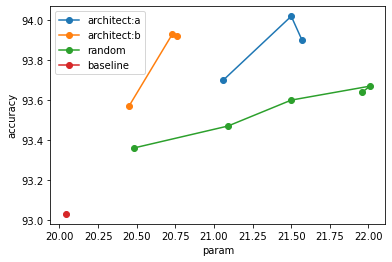
\includegraphics[clip,width=75mm]{param.png}
 		\caption{パラメータ数に対する精度}
 		\label{fig:param}
 	\end{center}
 \end{minipage}
 \begin{minipage}{0.5\hsize}
 	\begin{center}
 		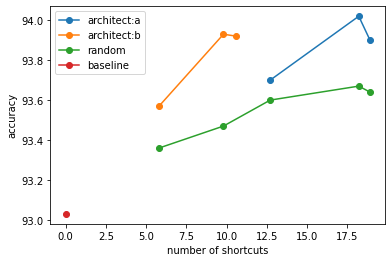
\includegraphics[clip,width=75mm]{short.png}
 		\caption{ショートカット数に対する精度}
 		\label{fig:short}
 	\end{center}
 \end{minipage}
\end{figure*}


\section{GAの準備}
deapでサンプルのGAを動作を確認.

問題
\begin{itemize}
  \item 個体表現($\alpha$は行列)
  \item 交叉・突然変異の方法
  \item メモリに乗るか?
  \item 実行時間
\end{itemize}
とりあえず今のDARTSのコードに実装してみる.

\section{事前学習実験}

DARTSは$w$を近似しているので高速である.
ベースモデルをVGGにはImageNetの事前学習モデルがある.
この重み$w$を利用するとより高性能なアーキテクチャが得られる?

\subsection{探索}
試しに1回実験した.
図 \ref{fig:acc} には探索中のテスト精度を示した.
これによると初期段階から高い精度が得られているため, ファインチューニングできている.

図 \ref{fig:graph_s}, \ref{fig:graph_e}, \ref{fig:graph_p}にはファインチューニングによる具体的なアーキテクチャの違いを図示した.
図 \ref{fig:alpha}, \ref{fig:alpha_p}には探索の結果の$\alpha$を示した.
図 \ref{fig:alpha_p}では, ファインチューニングによってより深い層でショートカットが必要になっている.

図 \ref{fig:graph_e}, \ref{fig:graph_p} では4ブロック以上離れた位置のショートカット数が多い.
手法AよりBの方が性能が高かったため, \ref{fig:graph_p}はさらに高い性能となることが期待される.

\subsection{評価}
usagiサーバーで実験を回そうとするとエラーを吐いてからログインできなくなった??

\begin{figure}[tb]
 	\begin{center}
 		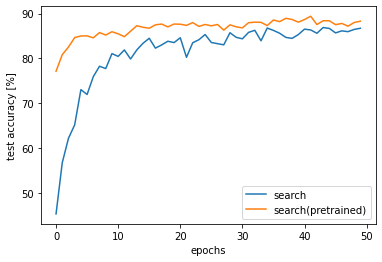
\includegraphics[clip,width=75mm]{acc.png}
 		\caption{$w$を事前学習した探索時のテスト精度}
 		\label{fig:acc}
 	\end{center}
\end{figure}

\begin{figure*}[tb]
 \begin{minipage}{0.333\hsize}
 	\begin{center}
 		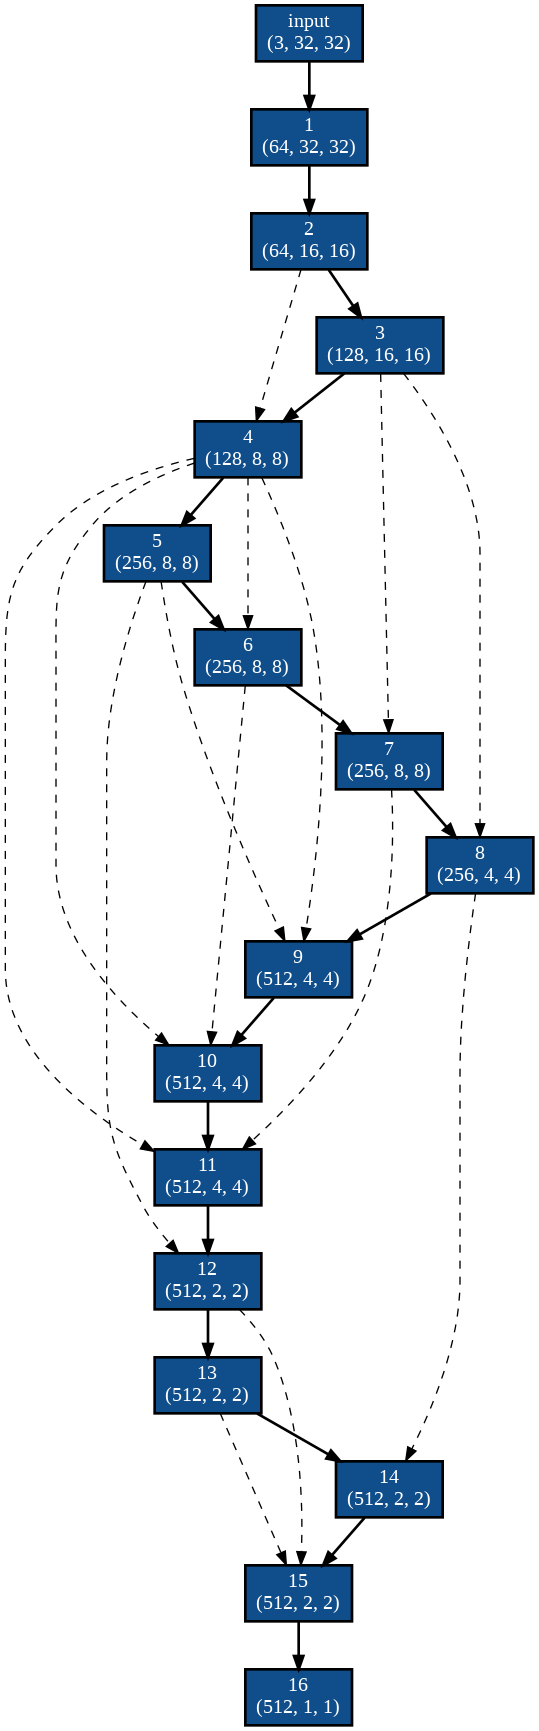
\includegraphics[clip,scale=0.25]{graph_50_search.png}
 		\caption{手法Aのグラフ(50 epoch)}
 		\label{fig:graph_s}
 	\end{center}
 \end{minipage}
 \begin{minipage}{0.333\hsize}
 	\begin{center}
 		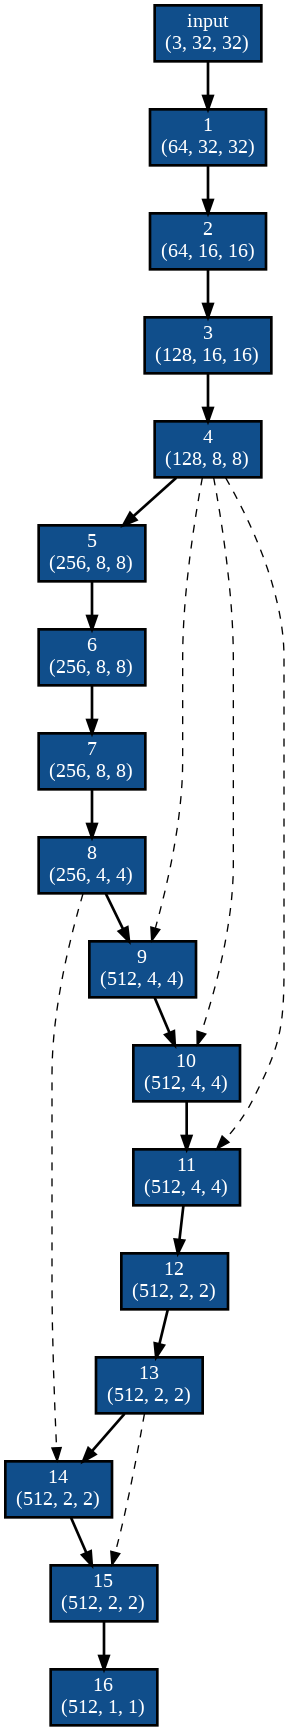
\includegraphics[clip,scale=0.25]{graph_50_search_edge.png}
 		\caption{手法Bのグラフ(50 epoch)}
 		\label{fig:graph_e}
 	\end{center}
 \end{minipage}
 \begin{minipage}{0.333\hsize}
 	\begin{center}
 		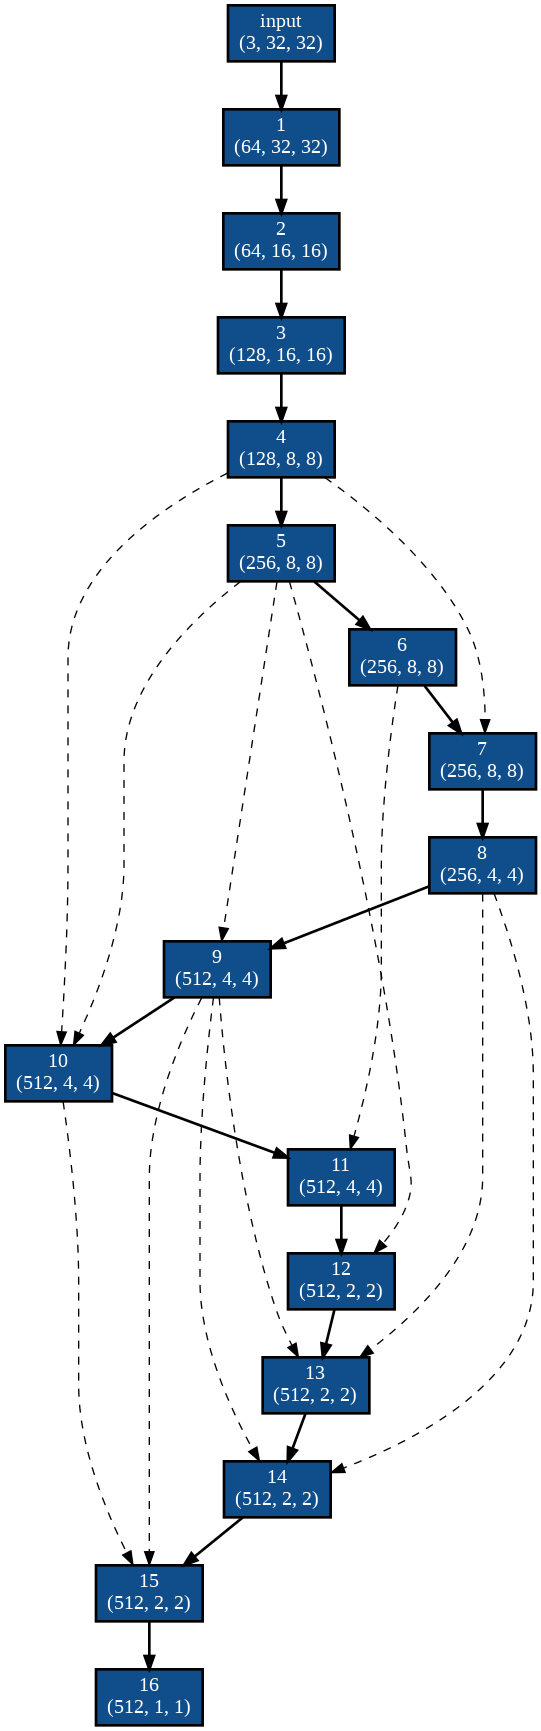
\includegraphics[clip,scale=0.25]{graph_50_pretrain_search.png}
 		\caption{手法Aのグラフ(50 epoch, pretrained)}
 		\label{fig:graph_p}
 	\end{center}
 \end{minipage}
\end{figure*}

\begin{figure*}[tb]
 \begin{minipage}{0.5\hsize}
 	\begin{center}
 		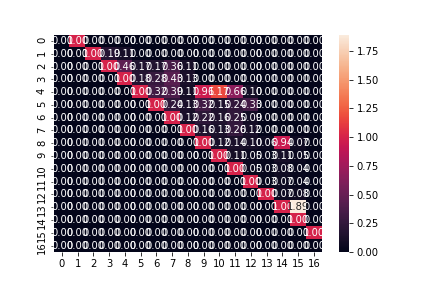
\includegraphics[clip,width=75mm]{alpha_50_search.png}
 		\caption{事前学習なしの$\alpha$(従来)}
 		\label{fig:alpha}
 	\end{center}
 \end{minipage}
 \begin{minipage}{0.5\hsize}
 	\begin{center}
 		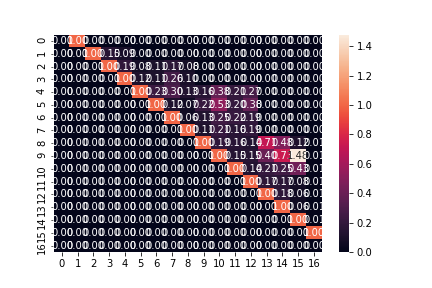
\includegraphics[clip,width=75mm]{alpha_50_pretrain_search.png}
 		\caption{事前学習ありの$\alpha$(今回)}
 		\label{fig:alpha_p}
 	\end{center}
 \end{minipage}
\end{figure*}

\section{今後の予定}
% なんとなくなんかの勉強をするとかではなく具体的に

\begin{itemize}
  % \item DARTのunrolling実験
  % \item バグの修正
  \item 評価実験回す
  \item できればGAの実装
  % \item 論文の調査
\end{itemize}

\section{ソースコード}
% 埋め込みでもGitでもいいので参照できるように
githubのnotebookリポジトリ参照.

% 参考文献リスト
\bibliographystyle{unsrt}
\bibliography{ref}
\end{document}
